\chapter{\textbf{Introduction}}

\label{Introduction}

Cloud computing has attracted a lot of attention lately. It was popularized as a business model by Amazon's Elastic Compute Cloud (EC2), which started selling virtual machines (VMs) in 2006. Over time, more cloud providers have appeared in the market, offering their computational resources (CPU, memory, and I/O bandwidth). This definition of cloud, in which the IT infrastructure is deployed through virtual machines, is referred as Infrastructure-as-a-service (IaaS). One of the most appealing benefits of this paradigm, when associated to cloud providers, is the ability to cut costs. Companies may base their IT strategies on cloud-based resources, spending very little or no money managing their own IT infrastructure. They pay for these resources on-demand, in contrast to the traditional resource provisioning model, in which they would need to deal with both under- and over- utilization of their own resources. Moreover, the cloud providers may offer lower prices because they are benefited from the economy of 
scale.


These gains are seen on public clouds -- clouds made available in a pay-as-you-go manner to the public by an external provider. Although the market has evolved around this type of cloud, organizations might build IaaS clouds using their own infrastructure, known as private clouds. Their aim is not to sell capacity  over the internet,  but to give local users an agile and flexible infrastructure to run service workloads in their administrative domains. These users are offered VMs, which are scheduled in a group of physical machines within their organization, which we call a cluster. This leads to a better utilization of resources, since services with little demand can be packed into the same machine, process known as server consolidation. This means that on private clouds there is also the possibility to cut IT costs, since the consolidation aims to minimize the number of physical servers needed. Other benefits, such as the migration of VMs between hosts and the ability to dynamically change the 
amount of resources provided to it, enabled by the  technology present in virtual machine monitors (VMMs), make it 
possible to deal with fluctuations in the workload. These characteristics propitiate an elastic environment, which is good for a private cloud, and vital for the pay-on-demand model used in public clouds.  It's also possible for an organization to mix these two types of clouds, creating a hybrid cloud,  which is useful to supplement a private cloud's infrastructure with external resources from a public one. However, this paper will focus on a private cloud environment. 

\section{Context}

A cloud is highly dependable on machine virtualization, essential to achieve its goals. Database management systems (DBMSes), like other software systems, are also increasingly being run on virtualized environments for many reasons. Some of them are mentioned in \cite{4498282}, \cite{4401021} and \cite{Soror:2008:AVM:1376616.1376711}, which include the reduction on the cost of ownership, better provisioning and manageability of applications and the ability to migrate them among physical hosts. Our paper is motivated by the possibility to take a variety of databases that run on dedicated computing resources and move them to a shared resource pool, on a private cloud, process known as \textit{Database Consolidation}. This scenario is discussed in \cite{instance1290}. This white paper gives a good example of how consolidation is applied in a production environment. It lists two deployment models in which this process may be performed onto a private cloud. 

In our paper, the deployment model considered is the \textit{Infrastructure Cloud} model, illustrated in figure  ~\ref{fig:infra-model}. In this model, there is generally a one-to-many relationship between servers and VM guests, considered by this paper. When a database service is requested, the whole operating system stack is built and provided. Elasticity in this model is limited. Although VM guests may be provided more virtual resources ( CPU or Memory ), they cannot span across servers ( i.e. they are limited to the resources from the server they are running on ). This means that the full resources of the private cloud cannot be brought to bear on a workload requirement. However, the guests will be able to benefit from the live migration feature, supported by most hypervisors, and thus be moved to a host with more resource availability. 

\begin{figure}[ht]
\centering
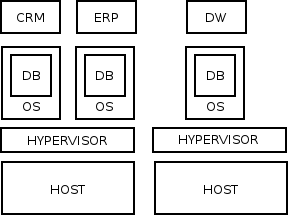
\includegraphics[width=0.5\textwidth]{infra-model.png}
\caption{Infrastructure cloud deployment model}
\label{fig:infra-model}
\end{figure} 

Some considerations should be made before adopting this deployment model. First, the virtualization won't reduce the number of DBMSes and operating systems, which will surely result in an overhead. It also won't probably be as high performing as other existing non-virtualized alternatives, as I/O intensive workloads may not perform as well in virtualized environments. However, it provides high fault and resource isolation, straightforward database deployment via VM templates and  support for multiple DBMS versions and configurations.


\section{Objective}

The problem addressed by our paper is formalized in \cite{4401021}, which defined it as the \textit{Virtualization Design Problem} (a.k.a. resource consolidation problem ) for relational database workloads. It can be defined as follows: \textit{"Given N database workloads that will run on N database systems inside virtual 
machines, how should we allocate the available resources to the N virtual machines to get the best overall performance?"}. According to the mentioned paper, this problem may find a better solution when applied to relational database systems due to three factors. First, relational database workloads consist of SQL queries with constrained and highly specialized resource usage patterns. Second , queries are highly variable in the way they use resources -- one query might heavily need CPU, while another might need I/O bandwidth instead. Thus, they could benefit from the dynamism in resource allocation. Third, database systems already have a way of modelling their own performance, namely the query optimizer.

As mentioned, DBMSes have particularities involving their workloads. Therefore, the application running inside a VM shouldn't be treated as a black box. Instead, the database system cost model should be exploited. As VMMs have parameters to control the share of physical resources, database systems also have tuning parameters to manage their own performance. These two sets need to be simultaneously analysed and tuned. In \cite{Soror:2008:AVM:1376616.1376711}, this is a principle of its proposed \textit{virtualization design advisor}. It works by recommending configuration parameters for a group of VMs, each one containing a DBMS. These parameters determine how the shared resources will be allocated to each VM, and consequently to each DBMS. It uses information about anticipated workloads to specify these parameters offline. Furthermore, runtime information collected after the deployment of the recommended configuration can be used to refine this recommendation and to handle fluctuations in the workload. This solution has 
not been proposed to run this advisor in a cloud yet, rather it has been implemented and tested in a single physical machine, in which two DBMS instances were deployed.

This paper demonstrates an implementation of the virtualization design advisor proposed in \cite{Soror:2008:AVM:1376616.1376711} in a cloud environment. Our objective is to solve the \textit{Virtualization Design Problem} in a distributed manner. Each node in a private cloud has its own corresponding instance of our advisor. Because of the \textit{Infrastructure model}, only the resources within the node are be allocated among the VM guests hosted there. Due to time limitations, this paper is restricted to the consolidation of CPU. However, it could be expanded to other types of resource on future work. 

The rest of this paper is structured as follows. Chapter ~\ref{chap:relwork} is used to discuss related work. In chapter ~\ref{chap:virtualization}, the \textit{virtualization design advisor} is described. Chapter ~\ref{chap:infrastructure} is used to show how a cloud infrastructure is managed. In section ~\ref{chap:implementation}, we show how the integration of the advisor within the cloud management system was implemented. Section ~\ref{chap:results} is used to show the results obtained. Finally, section 5 presents some final considerations and ideas for future work.

